% !TEXroot=main.tex
\section{Navigation}
{	
		\subsection{Costmap}
		{
			Die gegebene Karte wird in eine Costmap umgewandelt. Dabei bleibt die Grundfunktion bestehen. Eine Karte, welche Hindernisse aufzeigt. Zusätzlich dazu unterstützt diese Karte jedoch bei der Wegfindung. Jeder Punkt auf der Karte erhält einen Wert - dessen Kost, welche die Wahrscheinlichkeit eines Zusammenstoßes beschreibt. Ist diese Kost hoch, bedeutet dies, dass, sofern der Mittelpunkt des Roboters sich auf diesem Punkt befindet, eine Kollision mit einem Gegenstand sehr wahrscheinlich ist. Je weiter ein Punkt von einem Hindernis entfernt ist, desto geringer ist der Wert dieses Punktes. 
			\begin{figure}[H]
				\centering				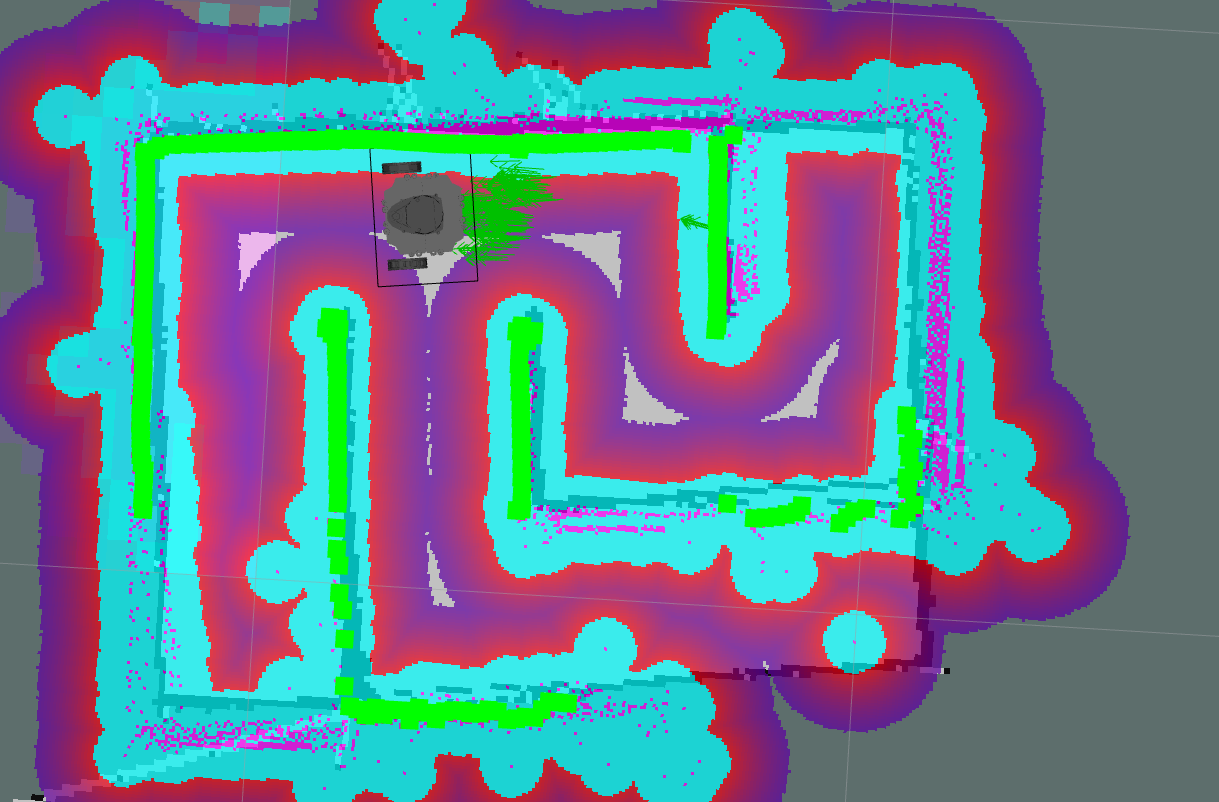
\includegraphics[height=5cm]{Bilder/costmap_overlayed.png}
				\caption{Die Costmap einer Karte} 
				\label{pic:costmapoverlayed}
			\end{figure}
			Die beigefügte Abbildung zeigt die Costmap. Es ist zu erkennen, dass der Bereich um Hindernisse (lila) verschieden gefärbt ist, was die abnehmenden Kosten für diesen Punkt beschreibt.
		}
	
		\subsection{Wegplanung}
		{
			Der zu befahrende Weg wird basierend auf mehreren Variablen geplant. Dazu zählt die Distanz im groben, \dahe der kürzeste Weg wird bevorzugt, aber auch gleichzeitig die Wahrscheinlichkeit einer Kollision während des Weges. Dazu werden die Kosten der Punkte auf der Costmap, welche auf dem Weg liegen betrachtet. Um mehr Variabilität bei der Wegplanung zu erlauben, wird die Planung in zwei Bereiche unterteilt. Ein globaler Planer plant den groben Weg zum Ziel, während ein lokaler Planer den Weg entlang des groben Weges plant, wobei gegebenenfalls auch Korrekturen vorgenommen werden müssen.
			
			\begin{figure}[H]
				\centering				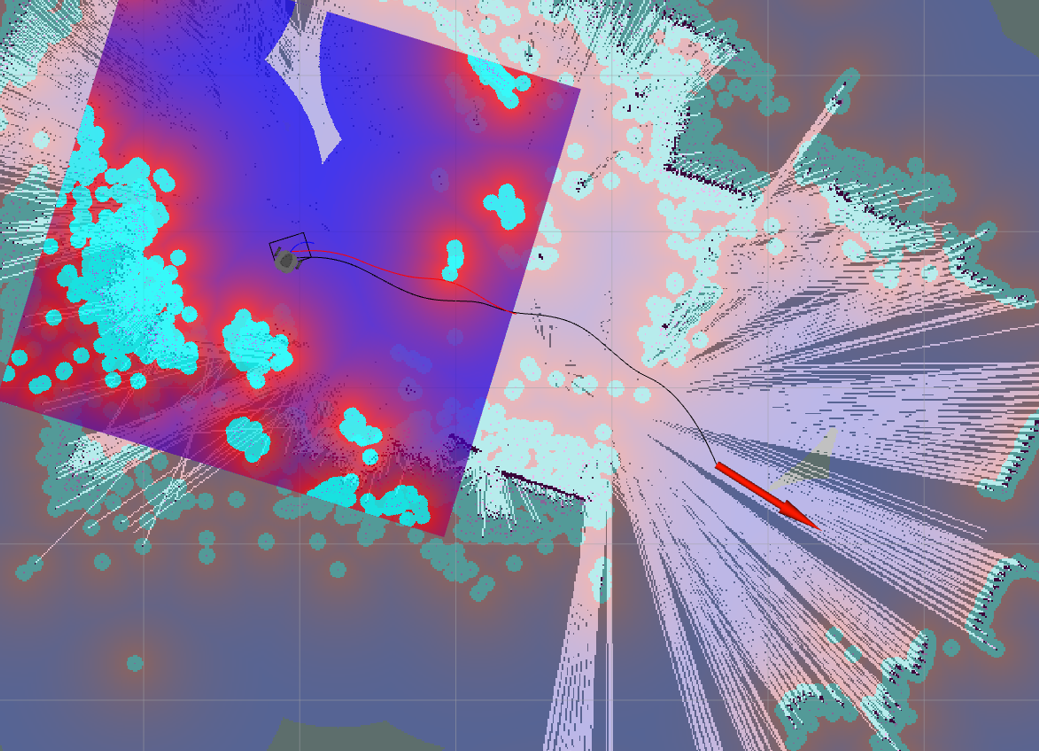
\includegraphics[height=5cm]{Bilder/costmap_pathplanning.png}
				\caption{Die Wegplaning, visualisiert in Rviz} 
				\label{pic:costpathplanning}
			\end{figure}
			
			Die obige Abbildung visualisiert den geplanten Weg. Dieser ist in einen roten, den lokal geplanten Weg, sowie einen Schwarzen, den global geplanten Weg aufgeteilt. Der blaue Strich repräsentiert die momentane Bewegungsrichtung. Weiter ist zu erkennen, dass die Costmap in einen lokalen Bereich (Rechteck), sowie einen globalen Bereich. Der lokale Bereich ist für die kurzfristige Wegplanung (lokaler Planer) für Bedeutung und hebt Hindernisse stärker hervor.
			
		}
		\subsection{Implementierung der Wegfindung} %https://www.researchgate.net/publication/253239158_ROSoClingo_A_ROS_package_for_ASP-based_robot_control
		{
			Um den Roboter nun zu einem Ziel zu navigieren, wird das move\textunderscore base-Package verwendet. Dieses steuert die Navigation des Roboters, sowie den Pfad, welchem der Roboter folgen soll. Es besteht aus mehreren Nodes (in der Abbildung oval dargestellt).  Dazu abonniert diese Nodes verschiedene Topics. Dazu gehören Sensordaten (z.B. sensor\textunderscore msgs/LaserScan für die Daten des LiDAR-Sensors), Odometriedaten und eine Karte. Die Karte wird durch einen Kartenserver bereitgestellt, welcher, als Node, diese Karte veröffentlicht, sodass jegliche Programme darauf zugreifen können. Dafür muss die Karte jedoch als Bild vorliegen, weshalb die Karte nach vollendeter Kartierung des Labyrinth auf einem Datenträger, meist die Festplatte eines über Wifi mit dem Turtlebot verbundenen Computers, gespeichert werden muss. Die gespeicherte Karte kann daraufhin von dem Karten-Server geöffnet werden. Dieses System sorgt gleichzeitig dafür, dass man eine Umgebung zur Navigation nicht notwendigerweise erneut kartieren muss, sollte schon eine Karte existieren. Im Anwendungsfall ist dies auch praktisch. Staubsageroboter müssen daher beispielsweise nicht jedes mal erneut eine komplette Karte eines Hauses erstellen.
			\begin{figure}[H]
				\centering
				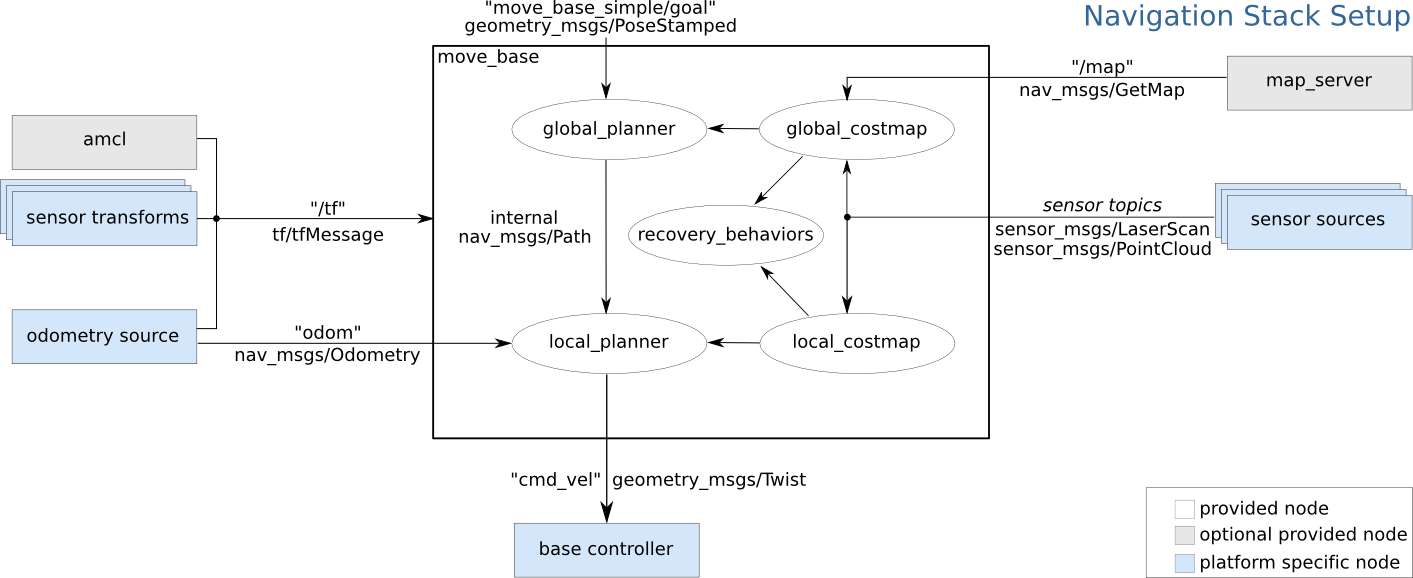
\includegraphics[height=7cm]{Bilder/overview_move_base.png}
				\caption{Das move\textunderscore base-Package \\
					\parencite{movebasenodeoverview}} 
				\label{pic:overviewmovebase}
			\end{figure}
			
			Nachdem der Roboter nun auf der durch den Kartenserver bereitgestellten Karte verordnet ist, muss dem Roboter ein Navigationsziel gegeben werden.
			Dazu gibt es mehrere Möglichkeiten. Das Programm Rviz ermöglicht es, wie bereits erwähnt, die Karte zu visualisieren. Gleichzeitig hat dies den Nebeneffekt, dass man durch das Programm bestimmen kann, welche Koordinaten ein Punkt auf der Karte hat, indem man die Maus auf diesen Bewegt. Rviz ermöglicht es sogar, direkt im Programm ein Navigationsziel festzulegen, was jedoch teilweise von dem Roboter nicht akzeptiert wird, weshalb ich ein Skript nutze, um die Koordinaten des Zielpunktes, welche ich in Rviz ablesen kann, an das move\textunderscore base-Package zu übertragen.
			Dafür wird folgendes Skript verwendet, in welchem der Roboter sich beispielhaft zu dem Punkt $P(3|2)$ bewegen soll:
			\newline  %https://answers.ros.org/question/80646/python-sending-goals-to-the-navigation-stack/
			
			\lstset{
				breaklines = true,
				frame = single,
				numbers = none
			}
			\begin{lstlisting} [language=Python]
01 import actionlib
02 import rospy
03 from move_base_msgs.msg import MoveBaseAction, MoveBaseGoal,   MoveBaseFeedback, MoveBaseResult
				
04 rospy.init_node("nav_goal_sender")
				
05 client = actionlib.SimpleActionClient("/move_base", MoveBaseAction)
06 client.wait_for_server()
				
07 goal = MoveBaseGoal()
08 goal.target_pose.header.frame_id = 'map' 
09 goal.target_pose.pose.position.x = 3
10 goal.target_pose.pose.position.y = 2
11 goal.target_pose.pose.orientation.z = 0
12 goal.target_pose.pose.orientation.w = 0.5
				
13 client.send_goal(goal)
14 client.wait_for_result()
				
			\end{lstlisting}
			Nun erläutere ich das Programm kurz Stück für Stück.
			Mit Hilfe der \textbf{import}-Befehle werden Bibliotheken eingebunden (Z. 1-3), welche Funktionalitäten für das Programm beinhalten, welche benötigt werden. Dazu zählt z.B: \textbf{rospy} (Z.2), welches eine Interaktion mit dem ROS-Betriebssystem ermöglicht, sowie verschiedene Klassen  \footcite{Programmierung: Ansammmlung von wiederverwandbaren Funktionen (eines Aufgabenbereiches)}, welche mit dem move\textunderscore base-Package zusammenhängen (Z.3).
			
			Daraufhin wird eine Node-initiiert, deren einzige Funktion ist, ein Navigatinsziel auszusenden. Die Node erhält den Namen "\textit{nav\textunderscore goal\textunderscore sender}" (Z.4).
			
			In den nächsten zwei Zeilen wird ein "Action-Client" \space initiiert. Dies ist eine Klasse, welche es ermöglicht, eine Action an einen Service auszusenden. Diese Art des Datenaustausches wurde in Abschnitt 2.1.5 - "Services" ausgeführt. Die Initiierung bedeutet vereinfacht gesagt, dass alles vorbereitet wird, sodass ein Befehl an den Service des move\textunderscore base-Packetes gesendet werden kann (Z.5f.).
			
			In den nachfolgenden sechs Zeilen (Z.7-12) werden die Parameter gesetzt, welche die Position, zu welcher Navigiert werden soll, bestimmen. Hier ist die z-Koordinate irrelevant, da der Roboter sich nicht nach oben/unten bewegen kann. Die x Koordinate (Z.9) wird gleich drei gesetzt. Die y-Koordinate gleich 2 (Z.10). In Zeile 11 wird die Richtung, in welche der Roboter am Ende schauen soll, festgesetzt.
			
			In Zeile 13 wird eine Action, also der Befehl mit den eingestellten Parametern, hier sind dies die Koordinaten, an den move\textunderscore base Service geschickt, welcher daraufhin zu diesem Ziel navigiert.
			
			
			
		}
	}
}